{
  \renewcommand{\bginsert}{\hfill\smash{\raisebox{-0.2\paperheight}{\color{tud orange}%
  
\includegraphics[width=2\paperwidth]{tud-logo.pdf}}}\hfill}
  \setbeamercolor{background canvas}{bg=tud yellow}
  \section{Matplotlib\\plots}
}

\makeatletter
\begin{frame}{A bar chart}
  \if@fourier
    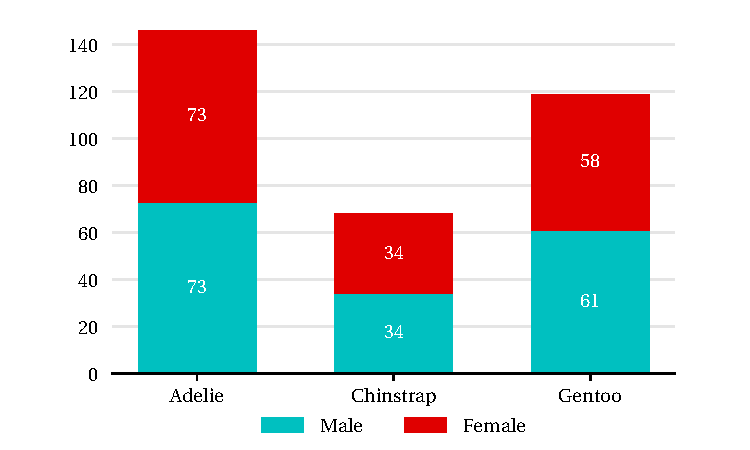
\includegraphics{_python/plt-bar-penguins_Utopia.pdf}
  \else
    \ifxetex
      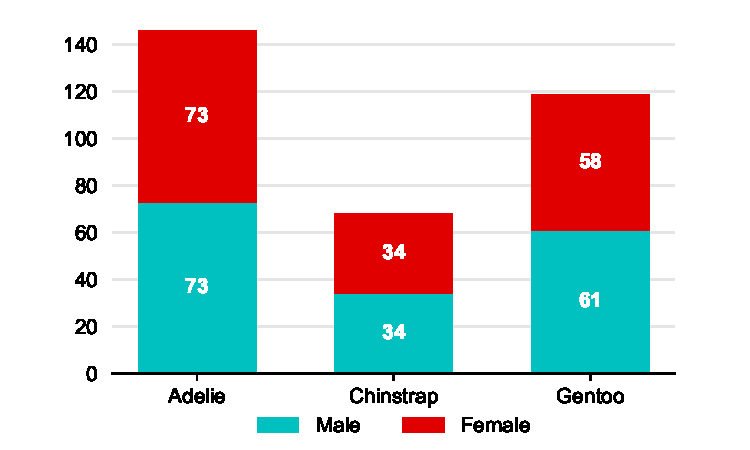
\includegraphics{_python/plt-bar-penguins_Arial.pdf}
    \else
      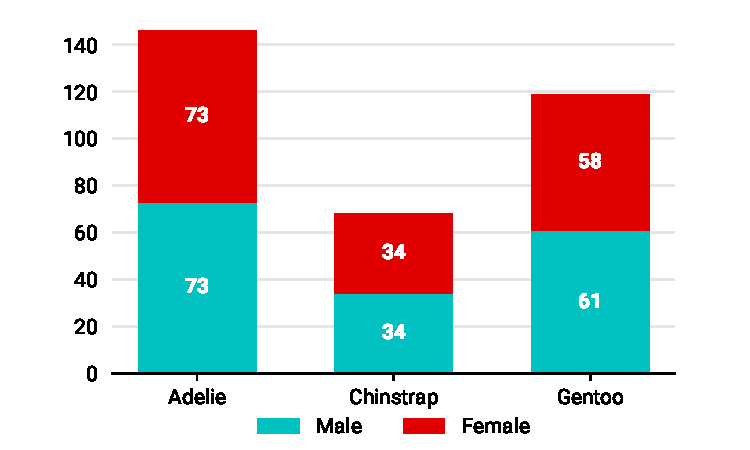
\includegraphics{_python/plt-bar-penguins_Roboto.pdf}
    \fi
  \fi
\end{frame}


\begin{frame}{A pie chart}
  \if@fourier
    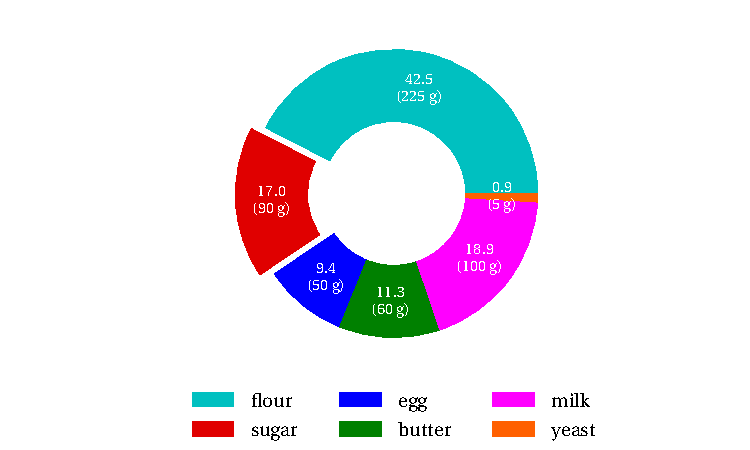
\includegraphics{_python/plt-pie-chart_Utopia.pdf}
  \else
    \ifxetex
      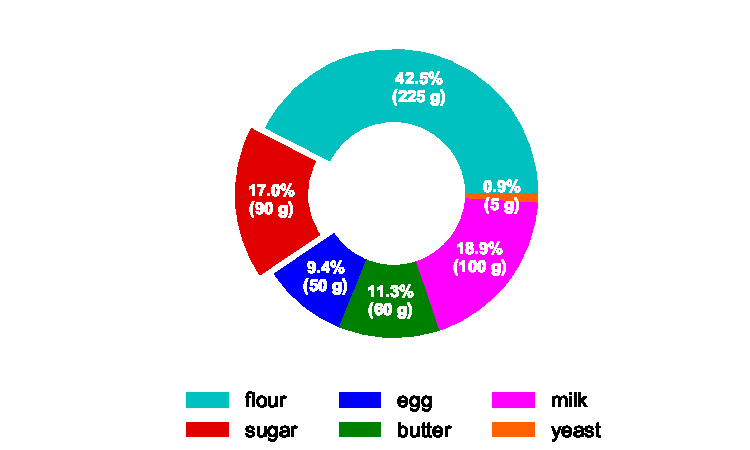
\includegraphics{_python/plt-pie-chart_Arial.pdf}
    \else
      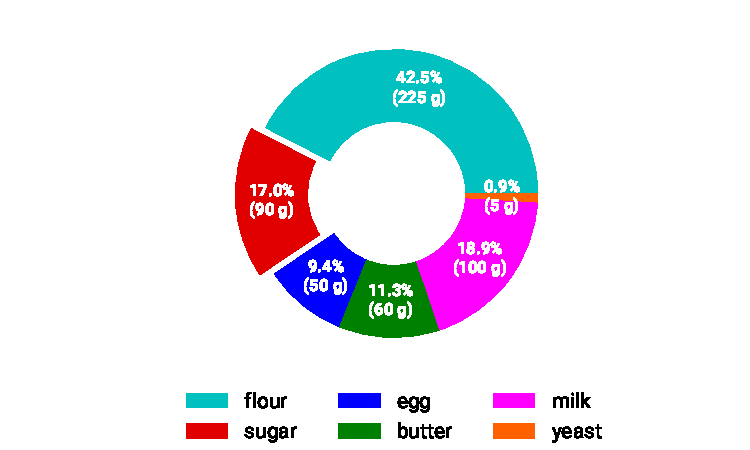
\includegraphics{_python/plt-pie-chart_Roboto.pdf}
    \fi
  \fi
\end{frame}


\begin{frame}{Confidence intervals}
  \if@fourier
    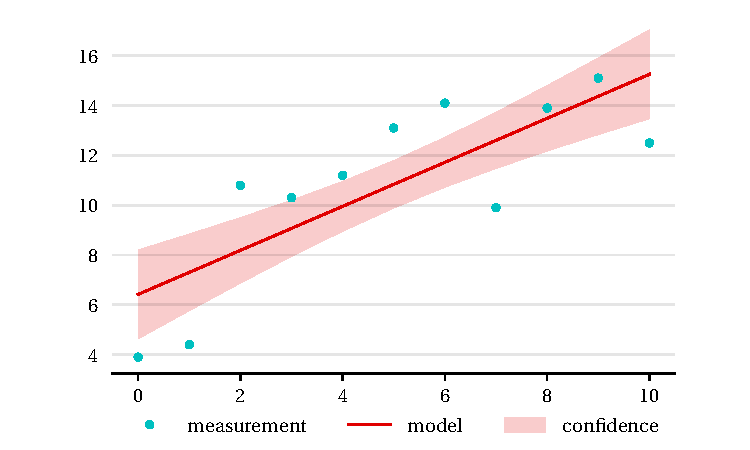
\includegraphics{_python/plt-confidence-bands_Utopia.pdf}
  \else
    \ifxetex
      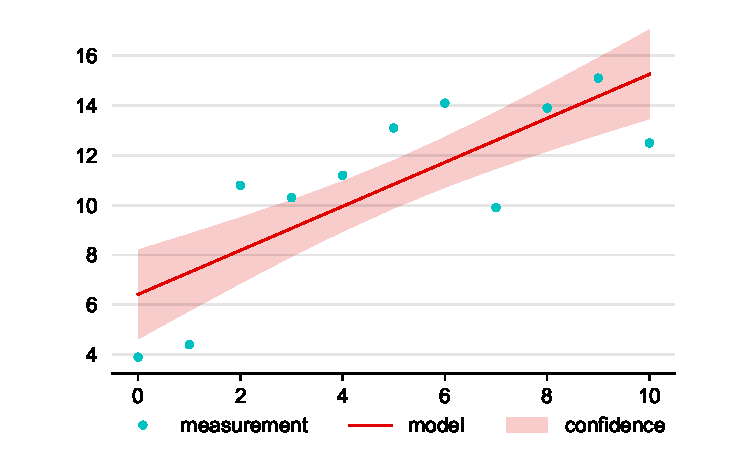
\includegraphics{_python/plt-confidence-bands_Arial.pdf}
    \else
      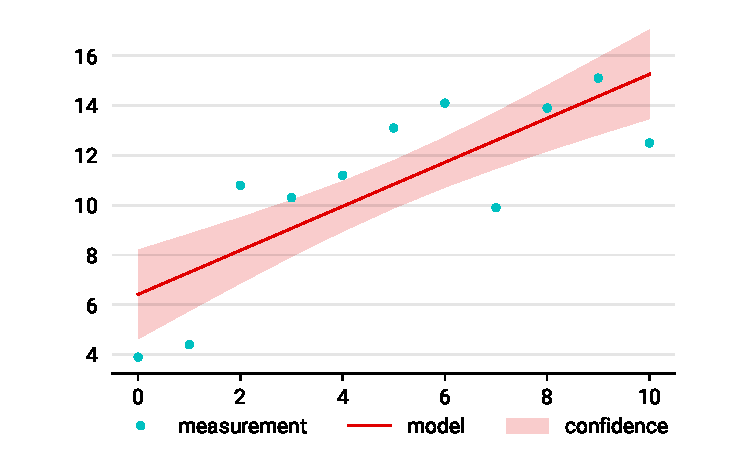
\includegraphics{_python/plt-confidence-bands_Roboto.pdf}
    \fi
  \fi
\end{frame}


\begin{frame}{Stream plot}
  \if@fourier
    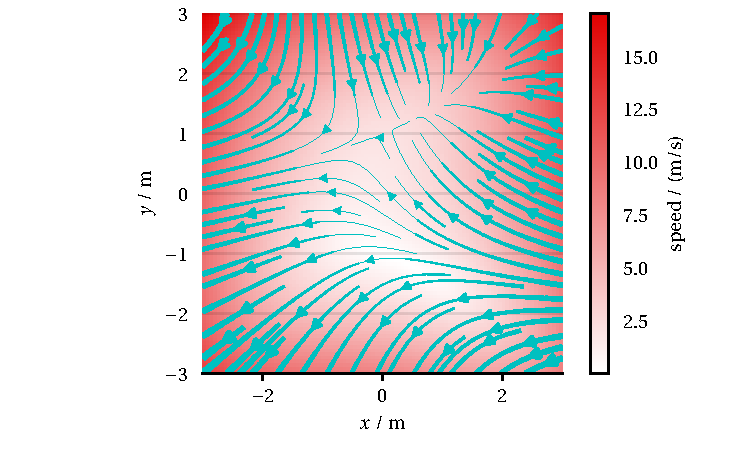
\includegraphics{_python/plt-streamplot_Utopia.pdf}
  \else
    \ifxetex
      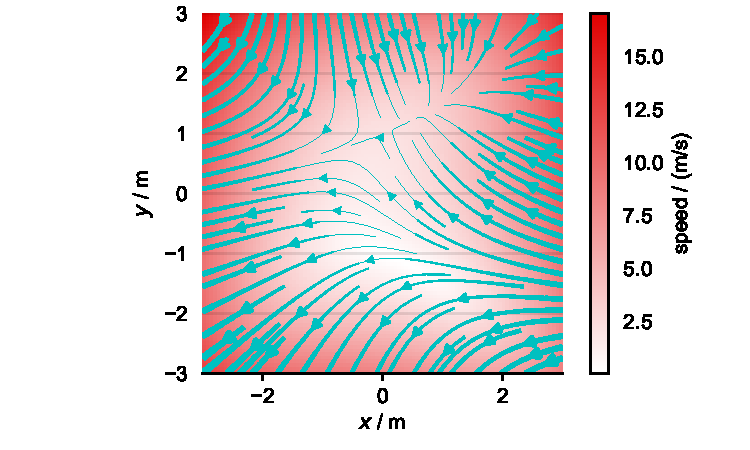
\includegraphics{_python/plt-streamplot_Arial.pdf}
    \else
      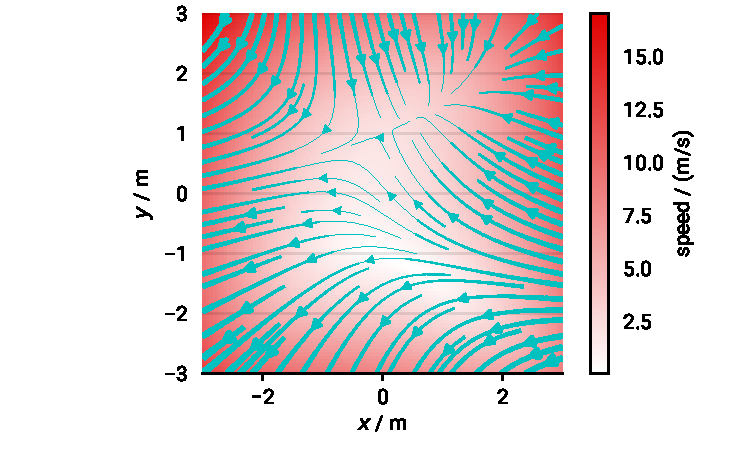
\includegraphics{_python/plt-streamplot_Roboto.pdf}
    \fi
  \fi
\end{frame}
\makeatother
